\documentclass[11pt]{article}

\usepackage[T1]{fontenc}
\usepackage[utf8]{inputenc}
\usepackage{amsmath,amssymb,amsthm}
\usepackage{graphicx}
\usepackage{booktabs}
\usepackage{xcolor}
\usepackage{tikz}
\usetikzlibrary{arrows.meta,positioning,calc,decorations.pathmorphing}
\usepackage[margin=1in]{geometry}
\usepackage{hyperref}
\hypersetup{hidelinks}

% One accent colour means "selected / active / observed". Grey means everything else.
\definecolor{accent}{HTML}{D97706}
\definecolor{quiet}{gray}{0.5}

% ---- notation ----
\newcommand{\R}{\mathbb{R}}
\newcommand{\C}{\mathbb{C}}
\newcommand{\CP}{\mathbb{CP}}
\newcommand{\RP}{\mathbb{RP}}
\newcommand{\Zt}{\mathbb{Z}_2}
\DeclareMathOperator{\softmax}{softmax}
\newcommand{\topm}[1]{\text{top-}#1}
\DeclareMathOperator{\cat}{cat}
\DeclareMathOperator{\atlas}{atlas}
\DeclareMathOperator{\Cayley}{Cayley}
\newcommand{\ket}[1]{\lvert #1\rangle}
\newcommand{\bra}[1]{\langle #1\rvert}
\newcommand{\braket}[2]{\langle #1\vert #2\rangle}
\newcommand{\norm}[1]{\lVert #1\rVert}

\newtheorem{proposition}{Proposition}

% title glyph: ०   (U+0966 DEVANAGARI DIGIT ZERO; pdflatex without a Devanagari font fails on it)
\title{Asmodeous (zero): An Atlas of Tiny Predictive Charts Made Real by an Observer}
\author{Teerth Sharma\\ \texttt{teerths57@gmail.com}}
\date{}

\begin{document}
\maketitle

\begin{abstract}
A measurement is the one step of quantum mechanics that is not linear, and it is the step that makes something real. This paper takes that sentence as an engineering principle. The model is an \emph{atlas of many tiny predictive charts}, each with its own small coordinate system, laid over a fragmented geometry. A softmax \emph{observer} plays the part of the measurement: it decides which charts are read, and only the charts it reads are computed (``observed $\Rightarrow$ exists''). The observer's weights are a partition of unity, so the charts it reads glue into one higher-dimensional space, and the pattern of which charts are read together is a nerve whose homology is the topology the model has learned. The observer is closed into a loop in the manner of a closed timelike curve: it reads the predicted futures of its candidate charts before it commits, and commits to the choice that is consistent with the future it causes. In time, as in space, nothing is computed unless something happens: an event-driven clock fires only on deviation. The mathematics is quantum (linear superposition, then a measurement that breaks linearity) and the machine is a classical consumer GPU. The idea is built as one architecture, ASMODEOUS, assembled slot by slot from the best available part. Its state is a point of $\CP^{N-1}$ that carries its own phase. Its observer is a Parseval-frame POVM whose probabilities sum to one exactly and which includes an outcome for observing nothing. Its charts are gauge-fixed and exist only when read, its gluing maps are learned unitary gauge links, its dynamics are unitary, and its time-traveller is a damped fixed point that provably converges. Its two parents, OBSERVER-ATLAS (real charts under a softmax observer) and PHASE-SPHERE (amplitudes under a Born decider), run beside it as first-class candidates. Every slot has a preregistered ablation, and measurements against owned baselines at equal active FLOPs and equal parameters decide which part earns each claim. \textbf{[Results: pending VERDICT.md.]}

\end{abstract}

\noindent\textbf{Keywords:} observer, atlas of charts, partition of unity, lazy computation, Born rule, POVM, Chern number, holonomy, closed timelike curve, event-driven computation, JEPA.

\section{Introduction}\label{sec:intro}

Computation has a hidden assumption: that the whole state is always there, waiting. A transformer holds every token against every token. A dense network runs every weight on every input. A fixed-rate renderer draws every frame whether or not anything moved. The world does not work like this. A quantum system is a superposition until it is measured, and what is measured is a \emph{choice} of basis that the observer makes. The idea of this paper is to build a learner that is made the same way: \textbf{nothing is computed until it is observed, and the observer decides what is worth observing.}

Picture a sphere cut into patches (Figure~\ref{fig:observer}). Each patch is a small model of its own neighbourhood: a tiny predictor with its own few coordinates, valid only where it lives. No single patch covers the sphere, and no single coordinate system ever can; that is a theorem, not a preference. The sphere is understood only by many small charts that agree where they overlap. Over the patches sits one decider, a softmax. It looks at the situation, assigns weight to the patches, and lets the heavy ones become real. The rest stay as potential: zero cost, zero parameters touched.

That picture carries a chain of ideas, and each link gives the next its reason.
\begin{enumerate}
  \item \textbf{The observer.} Turing's watched-pot paradox, the quantum Zeno effect~\cite{misra1977zeno}, says that a system measured often enough is frozen. The observer is not a spectator. It is part of the dynamics, and a model of computation that leaves it out leaves out the one operation that decides anything.
  \item \textbf{Quantum mathematics as an abstraction.} Linear superposition, then a measurement that breaks linearity: that two-step structure runs on a classical GPU as complex linear algebra followed by a normalisation. No quantum hardware and no quantum claim are involved, only the mathematics.
  \item \textbf{Many tiny charts that become real only when observed.} The geometry is fragmented on purpose. Charts are cheap and numerous; compute is spent only on the few the observer chooses. Parameters scale with the number of charts and compute scales with the number \emph{observed}.
  \item \textbf{One architecture from the best parts.} ASMODEOUS fills each slot (state, observer, charts, gluing, dynamics, loop, readout, training) with the part that does that job best, whichever parent it comes from. OBSERVER-ATLAS (a real atlas under a softmax observer) and PHASE-SPHERE (a phase sphere under a Born decider, the design of the origin notes) are its parents and run beside it. A part that wins is kept; a part that loses is replaced.
  \item \textbf{The time-traveller.} The observer is a closed loop. It reads the predicted futures of its candidate charts, and commits only to a choice that is consistent with the future it causes.
  \item \textbf{Time laziness.} The same principle applies to the clock. Computation fires at events and idles in between, as in the A.E.T.H.E.R.\ event-driven architecture.
\end{enumerate}

That is the image the name carries. Asmodeus, king of demons, commands a legion, and the legion costs nothing until it is summoned: the king names a few, those few appear and act in their own small corner of the world, and the rest remain names. Here the legion is the atlas of charts, the summons is the observer's softmax, and the corner each one acts in is its chart.

The intended result is a model whose cost follows what matters, whose parameters grow without its compute growing, and whose learned structure can be \emph{read out as a topology} (an integer, a Betti vector, a holonomy) instead of being inferred after the fact. JEPA, mixture-of-experts and attention are vocabulary and baselines in this work, not constraints.

\paragraph{Contributions.} The paper builds and tests the following.
\begin{itemize}
  \item ASMODEOUS: one architecture with a Parseval-frame POVM observer (exact probabilities with $K>N$ outcomes, so laziness costs no approximation), gauge-fixed charts on $\CP^{N-1}$, learned unitary gauge links, unitary dynamics and a damped, provably convergent time-traveller loop (Section~\ref{sec:asmodeous}).
  \item OBSERVER-ATLAS: an atlas of tiny predictive charts with a gated softmax observer, lazy top-$m$ evaluation, gluing into a higher-dimensional latent space, and an online nerve readout (Sections~\ref{sec:maths} and~\ref{sec:method}).
  \item PHASE-SPHERE: complex amplitudes on a sphere of phases with a Born decider, gauge-fixed charts, and integer readouts (a lattice Chern number and Berry holonomy) (Section~\ref{sec:method}).
  \item HYBRID: the composition of the real charts, the coherent decider and the time-traveller loop, built so that each part has a limit in which it vanishes (Section~\ref{sec:method}).
  \item A closed-loop observer defined as a fixed point, with an amortised head that predicts its answer in one pass, and an event-driven clock that spends compute only on deviation.
  \item A suite of owned baselines (single JEPA, MoP-JEPA, chart auto-encoder JEPA, lazy chart auto-encoder JEPA, PEER-JEPA, a CEM planner), matched to the atlas at equal active FLOPs and equal parameters.
  \item A table of verified identities that the mathematics rests on (Section~\ref{sec:identities}).
  \item A preregistered measurement protocol, T0--T7 and TO1--TO7, with bars and kills written before any result exists (Section~\ref{sec:experiments}).
\end{itemize}

\section{ASMODEOUS: one architecture, the best part in every slot}\label{sec:asmodeous}

ASMODEOUS is not a committee of models. Each slot was filled by asking which candidate part does that one job best, and the winner was taken whichever parent it came from: PHASE-SPHERE gives the state, the charts and the topological readouts; OBSERVER-ATLAS gives laziness and gluing; the A.E.T.H.E.R.\ paper gives the adaptive measurement and the event clock; the CTC loop of the origin notes gives the observer its time-traveller. Every slot has a preregistered ablation that removes it at equal active FLOPs and equal parameters, so a win is credited to a slot only when that slot's ablation loses it.

\begin{figure}[h]
\centering
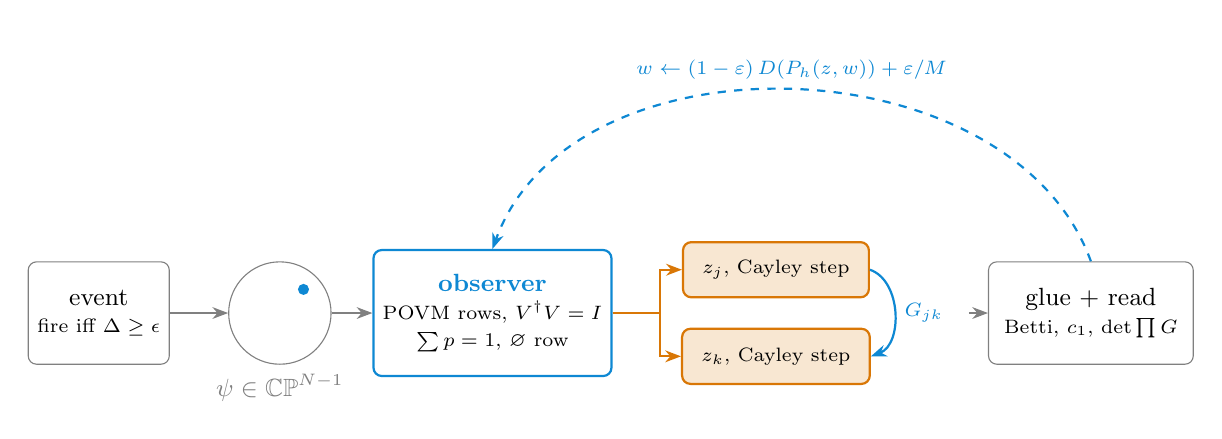
\begin{tikzpicture}[font=\small, >={Stealth[length=2mm]},
  box/.style={draw=quiet, rounded corners=3pt, minimum height=1.3cm, align=center},
  obs/.style={draw=cyan!70!blue, thick, rounded corners=3pt, minimum height=1.6cm, align=center},
  read/.style={draw=accent, thick, fill=accent!18, rounded corners=3pt, inner xsep=7pt, minimum width=1.9cm, minimum height=0.7cm, align=center}]
  \node[box, minimum width=1.5cm] (ev) at (0,0) {event\\[-1pt]\scriptsize fire iff $\Delta\ge\epsilon$};
  \node[circle, draw=quiet, minimum size=1.3cm] (psi) at (2.3,0) {};
  \fill[cyan!70!blue] ($(psi.center)+(0.3,0.3)$) circle (2pt);
  \node[below=0pt of psi, text=quiet] {$\psi\in\CP^{N-1}$};
  \node[obs, minimum width=2.4cm] (dec) at (5.0,0) {\textcolor{cyan!70!blue}{\textbf{observer}}\\[-1pt]\scriptsize POVM rows, $V^\dagger V=I$\\[-1pt]\scriptsize $\sum p=1$, $\varnothing$ row};
  \node[read] (zj) at (8.6,0.55) {\scriptsize $z_j$, Cayley step};
  \node[read] (zk) at (8.6,-0.55) {\scriptsize $z_k$, Cayley step};
  \node[box, minimum width=2.6cm] (glue) at (12.6,0) {glue + read\\[-1pt]\scriptsize Betti, $c_1$, $\det\prod G$};
  \draw[->, quiet] (ev) -- (psi);
  \draw[->, quiet] (psi) -- (dec);
  \draw[->, accent, thick] (dec.east) -- ++(0.6,0) |- (zj.west);
  \draw[->, accent, thick] (dec.east) -- ++(0.6,0) |- (zk.west);
  \draw[->, cyan!70!blue, thick] (zj.east) to[bend left=70] node[right, font=\scriptsize] {$G_{jk}$} (zk.east);
  \draw[->, quiet] ($(zj.east)!0.5!(zk.east)+(1.25,0)$) -- (glue.west);
  \draw[->, cyan!70!blue, thick, dashed] (glue.north) to[out=110, in=70] node[above, font=\scriptsize, text=cyan!70!blue] {$w\leftarrow(1-\varepsilon)\,D(P_h(z,w))+\varepsilon/M$} (dec.north);
\end{tikzpicture}
\caption{ASMODEOUS, one step. Amber: the charts read this step, the only ones that compute. Blue: the observer, its gauge links and its damped time-traveller loop. Grey: everything that costs nothing until it is called.}
\label{fig:asmodeous}
\end{figure}


\begin{table}[h]
\centering\small
\begin{tabular}{@{}p{2.6cm}p{8.6cm}p{3.2cm}@{}}
\toprule
Slot & Part chosen & From \\
\midrule
state & $\psi=\mathrm{normalise}(E(o))\in\CP^{N-1}$; the phase is part of the state & PHASE-SPHERE \\
observer & Parseval-frame POVM: rows $v_k$ of an isometry $V\in\C^{(K+1)\times N}$, $V^\dagger V=I$, one row for ``observe nothing'' & A.E.T.H.E.R., Born, Naimark \\
charts & $z_k=V_k^\dagger\psi\,e^{-i\arg\alpha_k}$, gauge-fixed, computed only when read & PHASE-SPHERE \\
laziness in $K$ & score $K{+}1$ effects, run the top-$m$ charts; their weights are exact & OBSERVER-ATLAS \\
laziness in time & event trigger, adiabatic re-route, per-chart send-on-delta & A.E.T.H.E.R. \\
gluing & learned gauge links $G_{jk}\in U(d_c)$ with a cocycle loss (a learned \v{C}ech cocycle) & origin, PHASE-SPHERE \\
dynamics & $\hat z_k=\Cayley(X_k(a))\,z_k$, unitary & PHASE-SPHERE \\
observer loop & damped fixed point (a contraction) with an amortised one-shot head & origin CTC \\
readouts & nerve Betti over $\Zt$, Chern $c_1$ from $\psi$, holonomy $\det\prod G$ & both parents \\
training & fidelity $1-\lvert\langle\hat\psi_{t+1},\psi^{\mathrm{tgt}}_{t+1}\rangle\rvert^2$; Haar test against collapse & origin, LeJEPA \\
\bottomrule
\end{tabular}
\caption{ASMODEOUS slot by slot. The full rationale and the ablation for every row are in \texttt{ASMODEOUS.md}.}
\end{table}

\paragraph{The observer.} A $K\times N$ isometry with $K>N$ is a tight frame, so its rows already form a POVM with more outcomes than dimensions (Naimark), and every probability is exact:
\begin{equation}\label{eq:parseval}
p_k=\big\lvert\langle v_k,\psi\rangle\big\rvert^2,\qquad \sum_{k=0}^{K}p_k=\psi^\dagger V^\dagger V\psi=1,\qquad \gamma=1-p_\varnothing,
\end{equation}
where $v_k$ is row $k$ of $V$, $p_\varnothing$ is the probability of the ``observe nothing'' row and $\gamma$ is the gate. No partition function appears, so the weights of the top-$m$ read charts are the numbers the dense model would compute: laziness costs no approximation.

\paragraph{The time-traveller.} Damping makes the self-consistency map a contraction,
\begin{equation}\label{eq:damped}
w\;\leftarrow\;(1-\varepsilon)\,D\big(P_h(z,w)\big)+\tfrac{\varepsilon}{M}\mathbf{1},\qquad \varepsilon>0,
\end{equation}
so the fixed point $w^\star$ exists, is unique, and is reached geometrically from any start. An amortised head is distilled to produce $w^\star$ in one pass, so the answer is available before the loop that defines it runs.

\paragraph{Training on $\CP^{N-1}$.} The prediction loss is the fidelity $1-\lvert\langle\hat\psi_{t+1},\mathrm{sg}\,\psi^{\mathrm{tgt}}_{t+1}\rangle\rvert^2$, which is invariant to a global phase and lives on the space the state lives on. Anti-collapse compares sliced $\lvert\langle u,\psi\rangle\rvert^2$ to its Haar law $\mathrm{Beta}(1,N-1)$, the uniform reference on $\CP^{N-1}$.

\paragraph{A control that may take a slot.} A single Hopf chart ($\psi\in S^3$ read by the Hopf map to $S^2$) is preregistered as a control with its own bar. If it covers $S^2$ without tearing, it becomes the ASMODEOUS chart for that space; a part that wins is kept.

The primitives of Eqs.~\eqref{eq:parseval} and~\eqref{eq:damped} are test-bound (Section~\ref{sec:identities}); the full model is built test-first against its contract.

% Results for ASMODEOUS: empty until VERDICT.md exists.

\section{Background}\label{sec:background}

\subsection{Why an observer?}

An observer is the point where a continuum of possibilities becomes one outcome. Quantum mechanics names the operation (measurement), attention names its classical cousin (softmax over keys), and the body gives the everyday example: an intention picks a goal, and the geometry of the body computes the path. In every case there is a small decider on top and a rich local mechanism below, and the decider only has to pick, not to compute.

The paradox that opens the project is that \emph{the more often a system is watched, the less it moves}. Rotate a spin by a half-turn in $N$ equal steps and measure after each step; the survival probability of the starting state is
\begin{equation}\label{eq:zeno}
  P_{\mathrm{surv}}(N)=\cos^{2N}\!\left(\frac{\pi}{2N}\right)\;\xrightarrow{\;N\to\infty\;}\;1,
\end{equation}
where $N$ is the number of measurements during the rotation and $P_{\mathrm{surv}}$ is the probability that every measurement finds the system still in its starting state~\cite{misra1977zeno}. The observer changes what the system does. This is the first sign that an observer is a dynamical object and not a readout.

\subsection{Prior art}

Every part of the design has a closest owner. Table~\ref{tab:prior} names what each owns and what this work adds on top. Each owner is a baseline, a source of vocabulary, and a point of comparison.

\begin{table}[t]
\centering
\small
\caption{Prior art: what each closest owner holds, and what the atlas adds.}
\label{tab:prior}
\begin{tabular}{@{}p{2.7cm}p{6.1cm}p{6.5cm}@{}}
\toprule
Work & What it owns & What the atlas adds \\
\midrule
MoP-JEPA~\cite{mopjepa} & A context-only softmax router over $K$ JEPA predictor heads on a shared encoder, with hard winner-take-all selection; fixes conditional-mean collapse. & A separate chart (encoder and embedding space) for every JEPA; lazy evaluation, so unselected charts cost nothing; gluing of charts into a higher-dimensional space; a topology readout from the observer. \\
Chart Auto-Encoders~\cite{schonsheck2019chartae} & Atlases of local charts with learned encoders, decoders and chart membership, for auto-encoding manifolds. & Predictive (JEPA) charts instead of reconstruction; an observer that routes among charts; lazy top-$m$ evaluation; online nerve topology. \\
POUnets~\cite{pounets} & Learned partitions of unity that glue local approximations, for regression. & Partition of unity as an observer over latent world-model charts; laziness; a nerve readout of the cover that was learned. \\
PEER~\cite{peer} & Retrieval of a few experts out of a very large pool by product keys; parameters grow while compute stays fixed. & Experts that are charts with their own coordinates, glued into one space, with the topology of their co-selection read out. \\
LeJEPA / SIGReg~\cite{lejepa} & An anti-collapse regulariser (SIGReg) for joint-embedding predictive learning. & SIGReg applied per chart and on the glued latent; observer competition as a second, independent anti-collapse mechanism, tested by ablation. \\
V-JEPA 2~\cite{vjepa2} & Action-conditioned latent world models used for planning by model-predictive control. & An observer that reads the predicted futures of candidate charts before committing: a closed-loop decider with a fixed-point condition. \\
Mixture-of-Depths~\cite{raposo2024mod} & Per-token dynamic allocation of compute across layers. & Allocation across charts and across time, with the allocation itself carrying a topological readout. \\
Mapper~\cite{singh2007mapper} & Post-hoc topological summary of a data cloud through a cover and its nerve. & The cover is learned online by the observer, so the nerve is read from the model while it runs. \\
\bottomrule
\end{tabular}
\end{table}

\section{Mathematical foundation}\label{sec:maths}

Every object below is implemented in the \texttt{atlas/} package of the accompanying code, and every identity is checked by a reference script and the test suite (Section~\ref{sec:identities}).

\subsection{Superposition, then a measurement that breaks linearity}

A state is a unit vector $\psi$ expanded in a basis $\{u_k\}$. Evolution is linear. The \emph{decider} is the Born rule, the one non-linear step:
\begin{align}
  \ket{\psi} &= \sum_k \alpha_k\,\ket{u_k}, \qquad \alpha_k=\braket{u_k}{\psi}, \label{eq:superposition}\\
  p_k &= \frac{\lvert\alpha_k\rvert^2}{\sum_j\lvert\alpha_j\rvert^2} = \softmax\big(2\log\lvert\alpha_k\rvert\big)_k. \label{eq:born}
\end{align}
Here $\alpha_k$ is the amplitude of $\psi$ along the chart gauge $u_k$ and $p_k$ is the probability of observing chart $k$.

\begin{proposition}[Born is a softmax over log-magnitudes]\label{prop:born}
For amplitudes $\alpha_k\neq 0$, $\lvert\alpha_k\rvert^2/\sum_j\lvert\alpha_j\rvert^2=\softmax(2\log\lvert\alpha_k\rvert)_k$.
\end{proposition}
\begin{proof}
$\lvert\alpha_k\rvert^2=\exp(2\log\lvert\alpha_k\rvert)$, and a softmax is the exponential normalised by its sum.
\end{proof}

The second line of~\eqref{eq:born} is therefore an exact identity. Softmax attention is a classical observer; the Born rule is its coherent form, and the two meet at one formula.

\subsection{Measurement as a POVM}

A measurement that can be rotated, and therefore learned, is a positive operator-valued measure:
\begin{equation}\label{eq:povm}
  E_k=U^\dagger \Pi_k\, U,\qquad \Pi_k=\ket{k}\bra{k},\qquad \sum_k E_k=U^\dagger\Big(\sum_k\Pi_k\Big)U=I,\qquad E_k\succeq 0,
\end{equation}
where $U$ is a unitary with learnable parameters, $\Pi_k$ is the fixed projector onto basis state $k$, and $E_k$ is the effect that selects outcome $k$. Completeness $\sum_k E_k=I$ holds for every value of the parameters, so the measurement stays valid while it learns, and $p_k=\langle\psi|E_k|\psi\rangle$. The unitary is parametrised by a Cayley transform of a skew-Hermitian generator $X$, $U=\Cayley(X-X^\dagger)$, which is unitary for every $X$.

\subsection{The softmax observer is a partition of unity; charts glue into \texorpdfstring{$\R^{D_g}$}{R\^{}Dg}}

The observer scores every chart against a query and normalises:
\begin{equation}\label{eq:pou}
  w_k(x)=\softmax_k\!\left(\frac{q(x)\cdot\kappa_k}{\sqrt d}\right),\qquad w_k(x)\ge 0,\qquad \sum_k w_k(x)=1,
\end{equation}
where $q(x)$ is the query computed from the context at input $x$, $\kappa_k$ is the learned key of chart $k$, and $d$ is the key width. The weights sum to one at every input, which is the definition of a partition of unity subordinate to the cover by chart domains. Keep the heaviest $m$ charts $S=\topm{m}(w)$ and renormalise. Chart $k$ encodes the observation into its own small coordinates $z_k=E_k(o)\in\R^{d_c}$, and a gluing map $\phi_k:\R^{d_c}\to\R^{D_g}$ with $D_g>d_c$ places it in the shared space:
\begin{equation}\label{eq:glue}
  g=\gamma\sum_{k\in S}\tilde w_k\,\phi_k(z_k),\qquad \tilde w_k=\frac{w_k}{\sum_{j\in S}w_j},
\end{equation}
where $\gamma\in[0,1]$ is a learned gate that lets the observer observe nothing (a causal softmax with no gate collapses onto a single token; see Section~\ref{sec:identities}), and $g$ is the glued latent. Predictions glue the same way:
\begin{equation}\label{eq:predglue}
  \hat g_{t+1}=\gamma\sum_{k\in S}\tilde w_k\,\phi_k\big(P_k(z_k,a_t)\big),
\end{equation}
with $P_k$ the tiny predictor of chart $k$ and $a_t$ the action. Figure~\ref{fig:glue} shows the construction and the nerve that results.

\begin{figure}[t]
  \centering
  % Charts glued by a partition of unity into R^{D_g}, and the nerve that results.
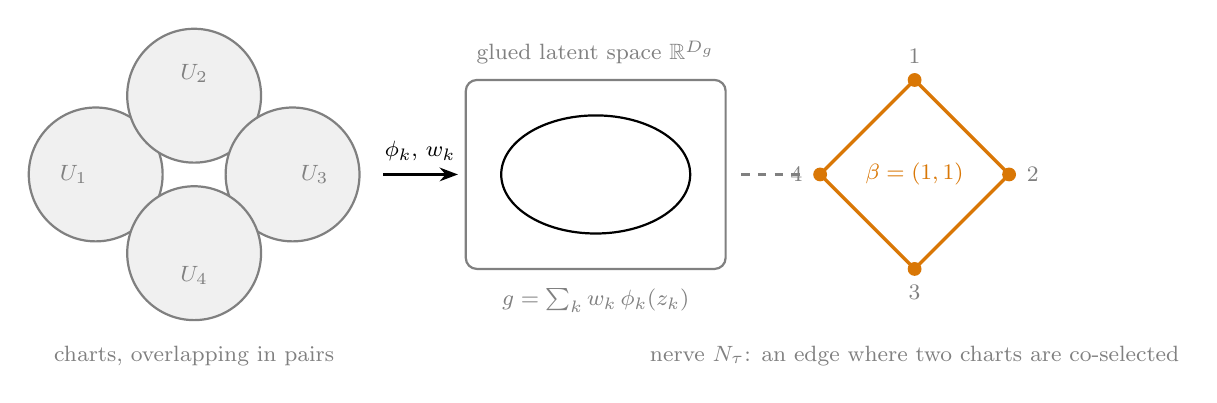
\begin{tikzpicture}[font=\footnotesize, >=Stealth]
  % four chart domains in a ring, overlapping in pairs
  \foreach \x/\y/\n in {0/0/1, 1.25/1/2, 2.5/0/3, 1.25/-1/4} {
    \draw[quiet, thick, fill=quiet!12] (\x,\y) circle (0.85);
  }
  \node[quiet] at (-0.28,0) {$U_1$};
  \node[quiet] at (1.25,1.28) {$U_2$};
  \node[quiet] at (2.78,0) {$U_3$};
  \node[quiet] at (1.25,-1.28) {$U_4$};
  \node[quiet] at (1.25,-2.3) {charts, overlapping in pairs};
  % gluing arrow
  \draw[->, thick] (3.65,0) -- (4.6,0);
  \node[above] at (4.12,0.05) {$\phi_k,\,w_k$};
  % glued latent space
  \draw[quiet, thick, rounded corners=4pt] (4.7,-1.2) rectangle (8.0,1.2);
  \draw[thick] (6.35,0) ellipse (1.2 and 0.75);
  \node[quiet] at (6.35,1.55) {glued latent space $\mathbb{R}^{D_g}$};
  \node[quiet] at (6.35,-1.6) {$g=\sum_k w_k\,\phi_k(z_k)$};
  % nerve
  \draw[quiet, dashed, thick] (8.2,0) -- (9.0,0);
  \begin{scope}[shift={(10.4,0)}]
    \draw[accent, very thick] (0,1.2) -- (1.2,0) -- (0,-1.2) -- (-1.2,0) -- cycle;
    \foreach \x/\y in {0/1.2, 1.2/0, 0/-1.2, -1.2/0} { \fill[accent] (\x,\y) circle (2.5pt); }
    \node[quiet] at (0,1.5) {1};
    \node[quiet] at (1.5,0) {2};
    \node[quiet] at (0,-1.5) {3};
    \node[quiet] at (-1.5,0) {4};
    \node[accent] at (0,0) {$\beta=(1,1)$};
    \node[quiet] at (0,-2.3) {nerve $N_\tau$: an edge where two charts are co-selected};
  \end{scope}
\end{tikzpicture}
\caption{Charts are glued by a partition of unity into the shared latent space $\mathbb{R}^{D_g}$, and the pattern of co-selected charts is a nerve. Four charts overlapping in pairs give a four-cycle, whose Betti vector over $\mathbb{Z}_2$ is $(1,1)$.}
\label{fig:glue}

\end{figure}

\subsection{The lazy rule: observed \texorpdfstring{$\Rightarrow$}{implies} exists}

Only the charts in $S$ run their encoder and predictor. Unselected charts are never read. The cost of a step is routing plus $m$ tiny charts:
\begin{equation}\label{eq:cost}
  C_{\text{step}}=C_{\text{route}}+m\,C_{\text{chart}},\qquad C_{\text{route}}=O(K\,d)\ \text{(flat keys)}\quad\text{or}\quad O(\sqrt K\,d)\ \text{(product keys)},
\end{equation}
where $K$ is the number of charts, $m\ll K$ the number observed, and $C_{\text{chart}}$ the cost of one tiny JEPA. The dense reference costs $K\,C_{\text{chart}}$. Parameters grow with $K$, compute does not. The lazy top-$m$ computation is checked against the dense mixture that zeroes the same weights (parity), and the unselected charts are checked to cost nothing (Section~\ref{sec:identities}).

\subsection{How many charts does a manifold need?}

No single chart covers a closed manifold without tearing (invariance of domain). With $\cat$ the Lusternik--Schnirelmann category and $\atlas(M)$ the least number of ball charts that cover $M$~\cite{rudyak2006atlas},
\begin{equation}\label{eq:atlasbound}
  \cat(M)+1\;\le\;\atlas(M)\;\le\;n+1,\qquad n=\dim M.
\end{equation}
By these bounds the sphere $S^n$ needs $2$ charts, the torus $T^2$ and the Klein bottle need $3$, and $SO(3)\cong\RP^3$ needs $4$. The atlas stops tearing at $K=\atlas(M)$, and not before. A rotation in $SO(3)$ has no continuous representation in four Euclidean dimensions or fewer, while five or six suffice~\cite{zhou2019rotation}, which is why the charts are glued into a space of higher dimension than their own.

\subsection{The nerve of the observer and its Betti numbers}

Charts that are read together form a simplicial complex. For a threshold $\tau$,
\begin{align}
  N_\tau&=\Big\{\sigma=\{k_0,\dots,k_r\}\;:\;\exists\,x\ \text{with}\ w_{k_i}(x)\ge\tau\ \ \forall i\Big\}, \label{eq:nerve}\\
  \beta_j&=\dim_{\Zt}H_j\big(N_\tau;\Zt\big). \label{eq:betti}
\end{align}
Here the vertices are the charts, a simplex is a set of charts co-selected with weight at least $\tau$ on some input, and $\beta_j$ is the $j$-th Betti number over $\Zt$. By the nerve theorem a good cover has the homotopy type of its nerve, so the learned topology can be read from the observer while the model runs, in contrast to a post-hoc cover-and-nerve summary~\cite{singh2007mapper}. Over $\Zt$ the targets are $S^2:(1,0,1)$, $T^2:(1,2,1)$ and $\RP^3:(1,1,1,1)$. A partition of unity places at most $\lfloor 1/\tau\rfloor$ charts above $\tau$, and a top-$m$ nerve has dimension at most $m-1$; both bounds are properties of the readout and are accounted for in its design.

\subsection{The phase sphere: amplitudes, transition phases, Chern number, holonomy}

The origin notes read ``jepa as a phase over higher dimensional $S^2$ sphere; small phases all around the sphere; the decider will be a softmax''. In this reading the state is a point of projective Hilbert space, $\psi\in\CP^{N-1}$ (the Bloch sphere $\CP^1=S^2$ is the first case), and the small phases are the $U(1)$ fibre. Each chart is a local gauge:
\begin{equation}\label{eq:gauge}
  \alpha_k=\braket{u_k}{\psi},\qquad z_k=V_k^{\dagger}\psi\,e^{-i\arg\alpha_k},\qquad \hat z_k=\Cayley\big(X_k(a)-X_k(a)^{\dagger}\big)\,z_k,
\end{equation}
where $u_k\in\C^N$ is the learned gauge of chart $k$, $V_k$ a learned frame, the factor $e^{-i\arg\alpha_k}$ fixes the gauge so that $g$ does not depend on the global phase of $\psi$, and $\hat z_k$ is the local unitary step driven by the action $a$ (a Cayley transform of a skew-Hermitian generator is unitary). Neighbouring gauges differ by a \emph{transition phase}:
\begin{equation}\label{eq:transphase}
  \chi_{jk}=\arg\big(\alpha_j\,\overline{\alpha_k}\big).
\end{equation}
The topological readout is an integer. For a triangulated sphere of states, take the link variables $U_{ab}=\braket{\psi_a}{\psi_b}/\lvert\braket{\psi_a}{\psi_b}\rvert$ and the plaquette field strength $F_\square=\arg\!\big(U_{12}U_{23}U_{31}\big)$ on the principal branch. The lattice \emph{Chern number} of Fukui, Hatsugai and Suzuki~\cite{fhs2005} is
\begin{equation}\label{eq:chern}
  c_1=\frac{1}{2\pi}\sum_{\square}F_\square,
\end{equation}
where the sum runs over the oriented triangles of the lattice and $c_1\in\mathbb Z$ up to an orientation convention. Its magnitude is $1$ for the Hopf bundle $S^3\to S^2$, the spin-$\tfrac12$ monopole, and $0$ for a trivial bundle. Along a closed path the same links give the \emph{Berry phase}, the holonomy of the state:
\begin{equation}\label{eq:berry}
  \gamma(C)=-\arg\prod_j\braket{\psi_j}{\psi_{j+1}},\qquad \gamma=-\tfrac12\,\Omega\ \ \text{(spin-$\tfrac12$)},
\end{equation}
where $C$ is the closed loop of states and $\Omega$ is the solid angle the loop encloses on the sphere. A transported frame returns with a sign $\pm1$ around the non-orientable loop of a Klein bottle and with sign $+1$ around every loop of a torus, so the holonomy sign separates the two surfaces at the level of individual loops.

\subsection{The closed loop: the observer as a fixed point}

The loop in the origin notes, the observer's closed timelike curve, is a self-consistency condition (Deutsch's condition $x=F(x)$~\cite{deutsch1991ctc}):
\begin{equation}\label{eq:fixedpoint}
  w^\star=D\big(P_h(z,\,w^\star)\big),\qquad w^{(i+1)}=D\big(P_h(z,\,w^{(i)})\big),\qquad \text{halt when } \norm{w^{(i+1)}-w^{(i)}}<\varepsilon,
\end{equation}
where $z$ is the current state, $w$ the observer's choice of charts, $P_h(z,w)$ the predicted state $h$ steps ahead when the charts $w$ are read, and $D$ the decider that maps a predicted future to a choice. The observer's choice must equal the choice it would make after seeing the future that choice causes. A continuous map of the simplex into itself always has a fixed point (Brouwer), so the loop always has an answer and there is no paradox. The G\"odel figure of the origin shows the same shape: the halting answer returns to the axis \emph{before} the start event (Figure~\ref{fig:ctc}). An \emph{amortised head} learns $\hat w(z)\approx w^\star(z)$ in one shot (trained by a KL divergence to the converged $w^\star$), so the answer exists before the iteration that defines it runs.

\subsection{The butterfly bonded by topology}

The continuous state may be chaotic while the integer readout stays put. With $J_t$ the Jacobian of the latent rollout at step $t$,
\begin{equation}\label{eq:lyapunov}
  \lambda_1=\frac1h\log\Big\lVert\prod_{t=1}^{h}J_t\Big\rVert
\end{equation}
is the finite-time largest Lyapunov exponent over the horizon $h$. The claim is that $\lambda_1>0$ (the continuous dynamics is sensitive) while the discrete readouts ($c_1$, the holonomy class, the Betti vector) cannot change under small perturbations unless a gap closes. The butterfly is bonded by topology.

\subsection{Event-driven time laziness (A.E.T.H.E.R.)}

The A.E.T.H.E.R.\ event-driven architecture renders a frame only when the scene has changed enough. With $\mu(t)\in\R^d$ the scene-feature vector, the deviation and the trigger rule are
\begin{equation}\label{eq:aether}
  \Delta(t)=\big\lVert\mu(t)-\mu(t-\delta t)\big\rVert_2,\qquad \text{fire iff }\ \Delta(t)\ge\epsilon,
\end{equation}
and the effective rate and the number of frames over a duration $T$ are
\begin{equation}\label{eq:fps}
  \mathrm{FPS}(t)\approx\frac{\lVert\dot\mu(t)\rVert}{\epsilon(t)},\qquad N_f=\int_0^T\mathrm{FPS}(t)\,dt\approx\int_0^T\frac{\lVert\dot\mu(t)\rVert}{\epsilon(t)}\,dt,
\end{equation}
where $\epsilon(t)$ is a threshold that the controller adapts, so the system raises it in noise and lowers it when motion matters. The same architecture defines the adaptive measurement as a POVM $E_k(\Phi)=U^\dagger(\Phi)\,\Pi_k\,U(\Phi)$ with $\sum_k E_k=I$ for every parameter $\Phi$, which is exactly the measurement of Equation~\eqref{eq:povm}. The two laziness axes compose: space decides \emph{which charts} run (Equation~\eqref{eq:cost}) and time decides \emph{at which instants} anything runs at all (Figure~\ref{fig:event}).

\begin{figure}[t]
  \centering
  % Event-driven time: compute only at events, idle between. Accent = events (compute), grey = everything else.
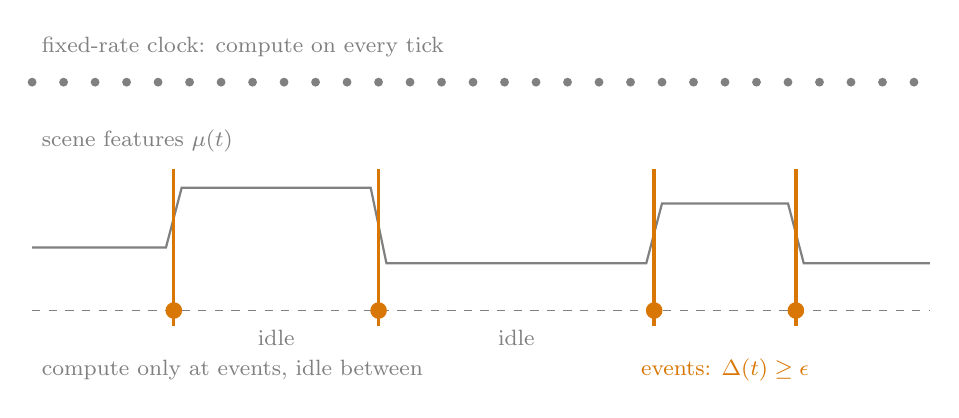
\begin{tikzpicture}[font=\footnotesize, >=Stealth]
  % fixed-rate clock: compute on every tick
  \node[quiet, right] at (0,4.55) {fixed-rate clock: compute on every tick};
  \foreach \i in {0,...,28} { \fill[quiet] (\i*0.4,4.1) circle (1.6pt); }
  % scene features
  \node[quiet, right] at (0,3.35) {scene features $\mu(t)$};
  \draw[quiet, thick] (0,2.0) -- (1.7,2.0) -- (1.9,2.76) -- (4.3,2.76) -- (4.5,1.8) -- (7.8,1.8) -- (8.0,2.56) -- (9.6,2.56) -- (9.8,1.8) -- (11.4,1.8);
  \draw[quiet, dashed] (0,1.2) -- (11.4,1.2);
  % events
  \foreach \x in {1.8,4.4,7.9,9.7} {
    \draw[accent, very thick] (\x,3.0) -- (\x,1.0);
    \fill[accent] (\x,1.2) circle (3pt);
  }
  \node[quiet] at (3.1,0.85) {idle};
  \node[quiet] at (6.15,0.85) {idle};
  \node[accent] at (8.8,0.45) {events: $\Delta(t)\ge\epsilon$};
  \node[quiet, right] at (0,0.45) {compute only at events, idle between};
\end{tikzpicture}
\caption{Event-driven time. A fixed-rate clock computes on every tick; the event-driven clock fires only when the scene deviation $\Delta(t)$ reaches the threshold $\epsilon$ (accent) and idles in between.}
\label{fig:event}

\end{figure}

\section{Method}\label{sec:method}

ASMODEOUS (Section~\ref{sec:asmodeous}) takes its parts from two parents, and both parents also run in full as first-class candidates on identical beds, seeds and metrics through one contract. A part that wins is kept and built on; a part that loses is replaced.

\subsection{OBSERVER-ATLAS}\label{sec:observer-atlas}

The atlas is $K$ tiny JEPAs with private charts (Figure~\ref{fig:observer}). Chart $k$ has an encoder $E_k:o_t\to z_k\in\R^{d_c}$ with $d_c$ small, a predictor $P_k:(z_k,a_t)\to\hat z_k$ in the same chart, a stop-gradient or EMA target encoder, and a gluing map $\phi_k$. A small causal backbone produces the context $c_t$, the observer turns it into the weights of Equation~\eqref{eq:pou}, a gate lets it observe nothing, and only the top-$m$ charts run (Figure~\ref{fig:lazy}). Charts are glued by Equations~\eqref{eq:glue} and~\eqref{eq:predglue}.

\begin{figure}[t]
  \centering
  % The observer choosing charts on a sphere. Accent = selected (top-m), grey = everything else.
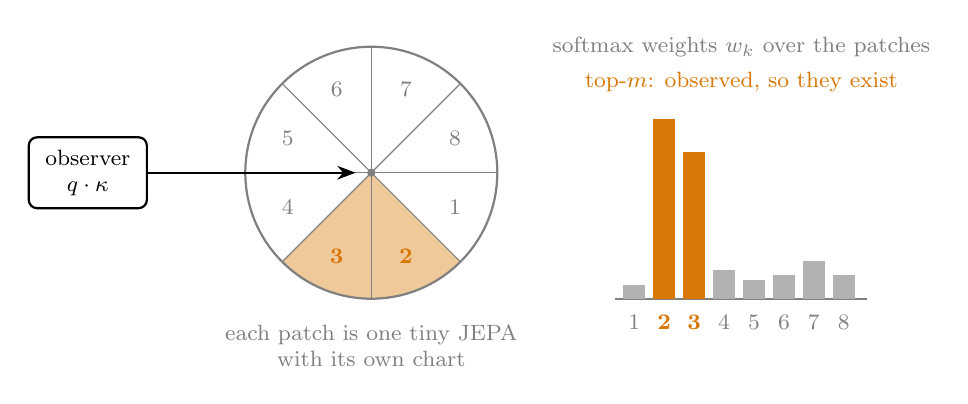
\begin{tikzpicture}[font=\footnotesize, >=Stealth]
  % sphere cut into 8 patches; patches 2 and 3 selected
  \def\R{1.6}
  \foreach \k in {2,3} {
    \pgfmathsetmacro{\a}{-(\k-1)*45}
    \pgfmathsetmacro{\b}{-\k*45}
    \fill[accent!40] (0,0) -- (\a:\R) arc (\a:\b:\R) -- cycle;
  }
  \draw[quiet, thick] (0,0) circle (\R);
  \foreach \k in {0,...,7} { \draw[quiet] (0,0) -- (-\k*45:\R); }
  \fill[quiet] (0,0) circle (1.5pt);
  \foreach \k in {1,...,8} {
    \pgfmathsetmacro{\m}{-(\k-0.5)*45}
    \ifnum\k=2 \node[accent, font=\footnotesize\bfseries] at (\m:1.15) {\k};
    \else\ifnum\k=3 \node[accent, font=\footnotesize\bfseries] at (\m:1.15) {\k};
    \else \node[quiet] at (\m:1.15) {\k};
    \fi\fi
  }
  % observer
  \node[draw, thick, rounded corners=3pt, minimum width=1.5cm, minimum height=0.9cm, align=center] (obs) at (-3.6,0) {observer\\$q\cdot\kappa$};
  \draw[->, thick] (obs.east) -- (-0.2,0);
  \node[quiet, align=center] at (0,-2.2) {each patch is one tiny JEPA\\with its own chart};
  % softmax weights
  \draw[quiet, thick] (3.1,-1.6) -- (6.3,-1.6);
  \foreach \h/\i in {0.18/1, 2.28/2, 1.86/3, 0.36/4, 0.24/5, 0.30/6, 0.48/7, 0.30/8} {
    \pgfmathsetmacro{\x}{3.2+(\i-1)*0.38}
    \ifnum\i=2 \fill[accent] (\x,-1.6) rectangle (\x+0.28,-1.6+\h); \node[accent, font=\footnotesize\bfseries] at (\x+0.14,-1.9) {\i};
    \else\ifnum\i=3 \fill[accent] (\x,-1.6) rectangle (\x+0.28,-1.6+\h); \node[accent, font=\footnotesize\bfseries] at (\x+0.14,-1.9) {\i};
    \else \fill[quiet!60] (\x,-1.6) rectangle (\x+0.28,-1.6+\h); \node[quiet] at (\x+0.14,-1.9) {\i};
    \fi\fi
  }
  \node[quiet] at (4.7,1.6) {softmax weights $w_k$ over the patches};
  \node[accent] at (4.7,1.15) {top-$m$: observed, so they exist};
\end{tikzpicture}
\caption{The observer chooses charts on a sphere. A softmax over the patches assigns weights $w_k$; the heaviest $m$ (here $m=2$, shown in the accent colour) are observed and therefore computed. The bar heights are illustrative.}
\label{fig:observer}

\end{figure}

\begin{figure}[t]
  \centering
  % Lazy compute: only the observed charts execute. Accent = observed, grey dashed = potential only.
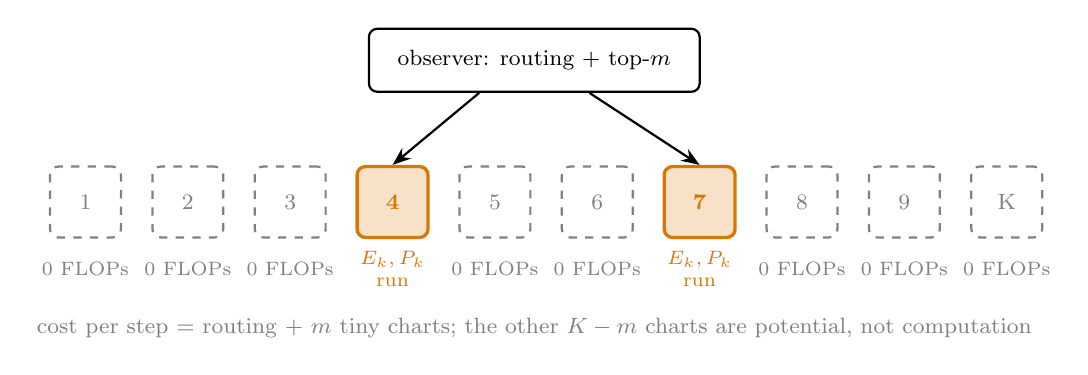
\begin{tikzpicture}[font=\footnotesize, >=Stealth]
  \node[draw, thick, rounded corners=3pt, minimum width=4.2cm, minimum height=0.8cm] (obs) at (6.3,2.4) {observer: routing + top-$m$};
  \foreach \i/\lab in {1/1,2/2,3/3,4/4,5/5,6/6,7/7,8/8,9/9,10/K} {
    \pgfmathsetmacro{\x}{0.6+(\i-1)*1.3}
    \ifnum\i=4
      \node[draw=accent, very thick, fill=accent!22, rounded corners=3pt, minimum size=0.9cm] (c\i) at (\x,0.6) {};
      \node[accent, font=\footnotesize\bfseries] at (\x,0.6) {\lab};
      \node[accent, align=center, font=\scriptsize] at (\x,-0.25) {$E_k,P_k$\\run};
    \else\ifnum\i=7
      \node[draw=accent, very thick, fill=accent!22, rounded corners=3pt, minimum size=0.9cm] (c\i) at (\x,0.6) {};
      \node[accent, font=\footnotesize\bfseries] at (\x,0.6) {\lab};
      \node[accent, align=center, font=\scriptsize] at (\x,-0.25) {$E_k,P_k$\\run};
    \else
      \node[draw=quiet, dashed, thick, rounded corners=3pt, minimum size=0.9cm] (c\i) at (\x,0.6) {};
      \node[quiet] at (\x,0.6) {\lab};
      \node[quiet, font=\scriptsize] at (\x,-0.25) {0 FLOPs};
    \fi\fi
  }
  \draw[->, thick] (obs.south) ++(-0.7,0) -- (c4.north);
  \draw[->, thick] (obs.south) ++(0.7,0) -- (c7.north);
  \node[quiet] at (6.3,-1.0) {cost per step = routing + $m$ tiny charts; the other $K-m$ charts are potential, not computation};
\end{tikzpicture}
\caption{Lazy compute. Only the observed charts (accent) run their encoder $E_k$ and predictor $P_k$; every unselected chart (dashed grey) costs zero FLOPs.}
\label{fig:lazy}

\end{figure}

The loss is the sum of: a per-chart JEPA loss against the stop-gradient target in the same chart, an overlap consistency term that makes co-selected charts agree in $\R^{D_g}$, a per-chart and glued-latent SIGReg term~\cite{lejepa}, a router load-balance term, and the task loss through $g$. Every structure the model uses (charts, routing, gluing, the manifold itself) is learned by SGD; hand-given structure scores as ``representable only'', never as ``works''. Anti-collapse is mandatory in every arm, because every self-supervised term here is minimised by a constant; the claim that observer competition alone limits collapse is tested only by ablation.

\subsection{PHASE-SPHERE}

The design of the origin notes is built as follows. The state is $\psi_t=\mathrm{normalise}(E(o_t))\in\C^N$. There are $K$ learned chart gauges $u_k$ and a null gauge $u_\varnothing$. A Born decider (Equation~\eqref{eq:born}) with a ``nothing'' outcome sets the gate $\gamma=1-p_\varnothing$. Lazy gauge-fixed charts $z_k$ are computed for the top-$m$ only, with a Cayley-unitary local dynamics (Equation~\eqref{eq:gauge}). The glued latent is $g=\gamma\sum_k\tilde w_k\,\phi_k([\mathrm{Re}\,z_k,\mathrm{Im}\,z_k])$, the transition phases are $\chi_{jk}$ (Equation~\eqref{eq:transphase}), and the closed-loop observer of Equation~\eqref{eq:fixedpoint} carries an amortised head. Its readouts are the Chern number of Equation~\eqref{eq:chern} and the Berry holonomy along held-out loops. Because amplitudes enter only through $K\cdot N$ Born scores, $K$ needs no product keys.

\subsection{HYBRID}

HYBRID is the composition of three parts: the real charts of OBSERVER-ATLAS; the coherent decider $p=\lvert U\psi\rvert^2$ with $\psi_k=\sqrt{\softmax(s)_k}\,e^{i\theta_k(q)}$ and $U$ a low-rank Cayley rotation; and the time-traveller loop (START preselects $M$ charts, the life-line rolls their candidate futures, HALT is the self-consistent set). Nothing is bound together by hand: every part has a limit in which it vanishes, and the arm starts at the first of those limits. \begin{equation}\label{eq:hybridlimits}
  \begin{aligned}
    \text{no coherence, no phase}&\ \Rightarrow\ \text{OBSERVER-ATLAS},\\
    \text{no loop}&\ \Rightarrow\ \text{coherent atlas},\\
    \text{no coherence}&\ \Rightarrow\ \text{time-traveller atlas}.
  \end{aligned}
\end{equation}
In the implementation the coherence parameters $C_p$ vanish in the no-coherence limit, and a loop gate $\gamma_{\mathrm h}$ (distinct from the observer gate of Equation~\eqref{eq:glue}) vanishes in the no-loop limit; the initialisation sits at the first limit, where $\theta$ has no effect. The hybrid contains OBSERVER-ATLAS, the coherent atlas and the time-traveller atlas as special cases, and learns how far from each to move. If the fixed-point observer of PHASE-SPHERE replaces the time-traveller loop, that is a recorded change made before any hybrid result, never a post-hoc pick between the two loops.

\subsection{The time-traveller}

The origin figure is the G\"odel-universe closed timelike curve (Figure~\ref{fig:ctc}): a life-line leaves the axis at START, spirals out to where the angular circles turn timelike, rides them backward in $t$, and returns to the axis at HALT, earlier than it left. In the architecture the life-line is the roll-out of candidate futures, and HALT is the self-consistent choice of Equation~\eqref{eq:fixedpoint}. The observer does not guess a chart and then find out. It reads what each candidate would predict and commits to the choice that survives its own prediction, and an amortised head learns to produce that choice in a single pass.

\begin{figure}[t]
  \centering
  % Left: the Goedel-style closed timelike curve, HALT below START on the t axis.
% Right: the observer reads three predicted futures and commits to the self-consistent one.
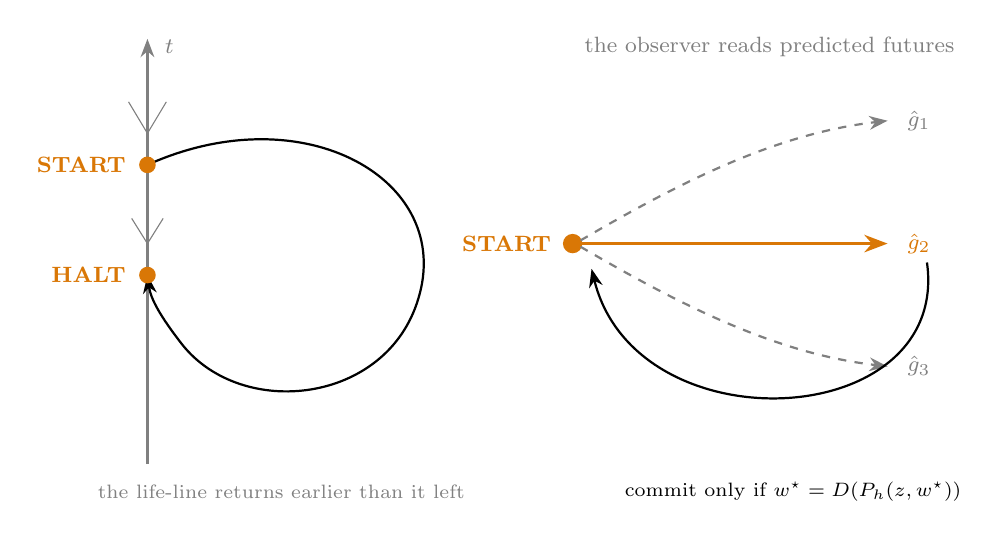
\begin{tikzpicture}[font=\footnotesize, >=Stealth]
  % ---- time axis and closed life-line ----
  \draw[quiet, thick, ->] (0,0) -- (0,5.4);
  \node[quiet, right] at (0.1,5.3) {$t$};
  \draw[thick, -{Stealth}] (0,3.8) .. controls (2,4.7) and (3.9,3.6) .. (3.44,2.1)
    .. controls (3.04,0.76) and (1.2,0.56) .. (0.44,1.52)
    .. controls (0.16,1.88) and (0.04,2.1) .. (0,2.4);
  \fill[accent] (0,3.8) circle (3pt);
  \fill[accent] (0,2.4) circle (3pt);
  \node[accent, left, font=\footnotesize\bfseries] at (-0.15,3.8) {START};
  \node[accent, left, font=\footnotesize\bfseries] at (-0.15,2.4) {HALT};
  % tipped light cones along the axis
  \draw[quiet] (0,4.2) -- (-0.24,4.6) (0,4.2) -- (0.24,4.6);
  \draw[quiet] (0,2.8) -- (-0.2,3.12) (0,2.8) -- (0.2,3.12);
  \node[quiet] at (1.7,-0.35) {\scriptsize the life-line returns earlier than it left};

  % ---- observer reading predicted futures ----
  \node[quiet] at (7.9,5.3) {the observer reads predicted futures};
  \fill[accent] (5.4,2.8) circle (3.5pt);
  \node[accent, left, font=\footnotesize\bfseries] at (5.25,2.8) {START};
  \draw[quiet, thick, dashed, -{Stealth}] (5.5,2.84) .. controls (6.8,3.6) and (8.0,4.2) .. (9.4,4.36);
  \draw[accent, very thick, -{Stealth}]   (5.5,2.8)  -- (9.4,2.8);
  \draw[quiet, thick, dashed, -{Stealth}] (5.5,2.76) .. controls (6.8,2.0) and (8.0,1.4) .. (9.4,1.24);
  \node[quiet]  at (9.8,4.36) {$\hat g_1$};
  \node[accent, font=\footnotesize\bfseries] at (9.8,2.8)  {$\hat g_2$};
  \node[quiet]  at (9.8,1.24) {$\hat g_3$};
  % commit loop back to START
  \draw[thick, -{Stealth}] (9.9,2.56) .. controls (10.2,0.4) and (6.2,0.2) .. (5.64,2.48);
  \node at (8.2,-0.35) {\scriptsize commit only if $w^\star = D(P_h(z,w^\star))$};
\end{tikzpicture}
\caption{The time-traveller. Left: a closed timelike curve in the G\"odel-universe picture; the life-line leaves the axis at START, rides back in $t$, and returns to the axis at HALT, earlier than it left. Right: the observer reads the predicted futures $\hat g_1,\hat g_2,\hat g_3$ of three candidate charts and commits only to the choice that is a fixed point of its own prediction.}
\label{fig:ctc}

\end{figure}

\subsection{Owned baselines and the matching rule}\label{sec:baselines}

Every owned method is a baseline, built to the same contract, trained by SGD, and matched to the atlas at \emph{equal active FLOPs and equal total parameters}. Active FLOPs are the multiply-accumulates per step of the observer's forward pass, and parameters exclude EMA copies; the atlas uses the same counting conventions. Each arm carries the shared SIGReg term and an EMA target, and takes only observations and actions as input. Table~\ref{tab:arms} lists the arms.

\begin{table}[t]
\centering
\small
\caption{The owned baselines and the role each plays.}
\label{tab:arms}
\begin{tabular}{@{}p{4.2cm}p{11.2cm}@{}}
\toprule
Arm & Role \\
\midrule
Single JEPA, several latent widths & The Whitney baseline: one chart wide enough to embed the manifold. \\
MoP-JEPA (dense and lazy)~\cite{mopjepa} & The closest owner: $K$ predictor heads on a shared encoder behind a context-only softmax router. \\
Chart-AE JEPA~\cite{schonsheck2019chartae} & Owner of separate charts and gluing, with membership over all $K$ charts. \\
Lazy chart-AE JEPA & The observer ablation: the atlas without the backbone, the gate and the keys. \\
PEER-JEPA~\cite{peer} & The owned route to ``parameters grow, compute stays fixed'' by product-key experts. \\
CEM planner & V-JEPA-2-AC-style~\cite{vjepa2} model-predictive control over any arm's rollout, with planning compute equalised across arms. \\
\bottomrule
\end{tabular}
\end{table}

The matching rule (L-BR) sizes each arm by its hidden width against the atlas's active FLOPs and parameters, with a tolerance of $\pm5\%$ on each axis. Two cases arise. When one configuration of the arm hits both targets, a single baseline runs (``both''). When the arm cannot hold the atlas's ratio of parameters to FLOPs, two baselines run: one at equal compute with fewer parameters (``flop''), and one at equal parameters with more compute (``param''). The atlas must beat each baseline on the axis it is matched on. Dense arms have parameters close to FLOPs, while top-1-of-$K$ arms have a parameter-to-FLOP ratio below $K$. A ``both'' match whose smallest width falls below $32$ is degenerate (for example a very narrow encoder feeding very wide heads) and is replaced by the split. Most of the atlas's active FLOPs sit in its causal backbone, and every owned arm spends that budget on encoder width instead.

Hyperparameters are tuned on a separate seed, with the same budget for every arm, the atlas included; widths are fixed by matching and never tuned. The selected configuration is frozen and trained on the evaluation seeds. The HYBRID arm is matched in the same way, with the coherent decider and its extra parameters counted, and its planning budget includes the coherent START decider and the worst-case loop cost.

Where an owned method is reimplemented, the deviations from its source are recorded. MoP-JEPA gains a SIGReg term because anti-collapse is mandatory in every arm (setting its weight to zero restores the paper-native arm, which the collapse test runs). Its unpublished hyperparameters are set by tuning, one prediction is read out at the router's top-1 head, and the latent width is set by matching rather than by the paper. Chart-AE JEPA replaces pixel reconstruction by JEPA losses against an EMA target, and the lazy variant adds top-$m$ routing with a load-balance term so that unselected charts keep a router gradient.

\section{Verified identities}\label{sec:identities}

Everything the mathematics stands on is a checked identity before it is a design. Every line of Table~\ref{tab:identities} is produced by the reference script \texttt{ref/identities.py} (pinned by SHA-256) or asserted by a passing test in the \texttt{tests/} directory of the accompanying code (eight test modules, covering the facts, the phase sphere, the coherent observer, contextuality, the observer atlas, the owned arms, topology, and the systems benchmark).

\begin{table}[t]
\centering
\footnotesize
\caption{Verified identities. The first column names the identity, the second its value, the third how it is checked.}
\label{tab:identities}
\begin{tabular}{@{}p{3.9cm}p{5.4cm}p{6.1cm}@{}}
\toprule
Identity & Value & Check \\
\midrule
Pin: SHA-256 of \texttt{ref/identities.py} & \texttt{467c2ae2\dots40a3fe} & matches the pin \\
Zeno: $\cos^{2N}(\pi/2N)$, $N=1,2,10,100,1000$ & $0.000000$, $0.250000$, $0.780546$, $0.975627$, $0.997536$ & simulated survival equal to 6 decimals \\
Born: $p=\softmax(2\log\lvert\alpha\rvert)$ & $=\lvert\alpha\rvert^2/\sum\lvert\alpha\rvert^2$ & atol $10^{-12}$, $100\times 9$ complex128 \\
L\"uders: $\max\lvert QQ\rvert$, pure and mixed states & $<10^{-14}$ & QQ equality holds \\
Classical: $\mathrm{mean}\lvert QQ\rvert$, with disturbance & $0.0751$ & QQ equality breaks \\
Softmax: causal stack, mass on token $1$ & $0.2543$ ($L=1$) $\to$ $1.0000$ ($L=16$) & reference script or test suite \\
IIA: $p_1/p_2$, key $3$ present / removed & softmax $1.3499$ / $1.3499$; coherent $g=1$: $2.0587$ / $1.3499$ & reference script or test suite \\
Cayley: $U^\dagger U=I$ & $50$ random generators & atol $10^{-10}$ \\
POVM: $\sum_k E_k=I$, $E_k\succeq 0$ & $K=N$ and Naimark $K>N$, 50 draws each & atol $10^{-10}$ (\texttt{tests/test\_povm.py}) \\
Frame: $V^\dagger V=I$, Stiefel retraction & $K\in\{16,65,257\}$ & $<10^{-10}$ (\texttt{tests/test\_asmodeous\_ops.py}) \\
Tight frame: $\sum p=1$ for $K>N$ outcomes & $p\ge 0$ & $<10^{-10}$ \\
Damped CTC loop: unique fixed point & 10 random starts & residual $<10^{-8}$; undamped cycle does not converge \\
Gauge links: $G_{jk}$ unitary, exact cocycle & random generators & $<10^{-10}$ \\
Parity: lazy top-$m$ $=$ dense masked mix & $K=8$ flat keys, $K=16$ product keys & atol $10^{-10}$ (float64) \\
Laziness & $g$, $\hat g$, loss unchanged (atol $10^{-12}$); dense control $\to$ NaN & unselected charts NaN-poisoned \\
FLOPs: active MACs, $m$ vs $K$ & per-chart cost exact in $m$; $K$ enters only the router & reference script or test suite \\
Kernel: fused Triton step $=$ \texttt{observe()} & $K=16\ldots4096$, flat and product keys & $10^{-4}$ \\
Berry: $\gamma=-\Omega/2$, spin-$\tfrac12$ latitude loops & $5/5$ latitudes; $200$ triangles exact to $10^{-9}$ & reference script or test suite \\
Chern: FHS lattice, levels $2,3,4$ & spin-$\tfrac12$ $-1$; spin-$1$ $-2$; trivial $0$ & reference script or test suite \\
Holonomy: transported sign & Klein $-1$; torus $+1$ & reference script or test suite \\
Fixed point: $w^\star=D(P(z,w^\star))$, $1000$ stochastic maps & residual $<10^{-8}$ & reference script or test suite \\
Betti $\Zt$: $S^2$, $T^2$, Klein, $\RP^3$ & $(1,0,1)$; $(1,2,1)$; $(1,2,1)$; $(1,1,1,1)$ & reference script or test suite \\
Betti $\mathbb Q$: $T^2$, Klein & $(1,2,1)$; $(1,1,0)$ & reference script or test suite \\
Nerve: top-$m$ readout, $20$ seeds & $\dim\le m-1$; PoU at $\tau$: $\dim\le\lfloor1/\tau\rfloor-1$ & reference script or test suite \\
\bottomrule
\end{tabular}
\end{table}

\section{Experiments}\label{sec:experiments}

Each claim of the project is a question put to a measurement. The beds, the bars and the kills are written into a preregistration file (\texttt{PREREG.md}) and committed before any result file exists, and every claim is scored for ASMODEOUS, its two parents and HYBRID under the same beds, seeds, matched sizes and owned baselines. The verdict for a claim names whichever candidate passes it. This section states the questions only; the bars live in \texttt{PREREG.md}.

\subsection{Measurement discipline}

Five rules govern every comparison. (L-GIVEN) Any structure that a bed supplies (charts, routing, gluing, manifolds, graphs) must be learned by SGD, and hand-given structure scores as ``representable only''. (L-PREREG) Beds, bars and kills are committed before any result exists; anything later is a post-hoc label. (L-BR) Baselines are the best owned methods at equal active FLOPs and equal total parameters, trained by SGD and tuned on a separate seed (Section~\ref{sec:baselines}). (L-WALD) A designed bed counts only if a neutral bed runs beside it. (L-LEARN) An arm must clear its in-distribution bar before it is compared. A literature gap is not a new primitive: novelty is earned only by a decisive test that the owned parts fail.

\subsection{Core tests}

\begin{description}
  \item[T0, reproduce.] Does the reference script reproduce its pinned output?
  \item[T1, owner hunt.] Is the full combination already owned? Every owned part is cited and used as a baseline.
  \item[T2, geometry (C1, C2).] On the sphere, torus, Klein bottle and $SO(3)$, with no manifold, chart or state ever given, does the atlas stop tearing at exactly $K=\atlas(M)$ with charts of the manifold's own dimension, and does the nerve recover the true Betti numbers online? A neutral flat bed runs beside them.
  \item[T3, lazy scaling (C3).] At fixed active compute, does loss fall as the number of charts $K$ grows, below a dense JEPA and below one JEPA with PEER experts? Does lazy top-$m$ stay within tolerance of the soft mixture over all $K$?
  \item[T4, collapse (C4).] With the anti-collapse regulariser weakened or removed, does observer competition keep the representation from collapsing? Does the atlas match MoP-JEPA on mode collapse on the OGBench pointmaze-stitch task?
  \item[T5, time-traveller (C5).] Does reading predicted futures before committing beat owned latent MPC at equal planning compute, on MuJoCo swing-up and OGBench pointmaze?
  \item[T6, contextuality.] Do query pairs show order effects and QQ-equality statistics as a quantum-structured observer predicts? Measurement only.
  \item[T7, systems.] Do lazy routing and tiny JEPAs run faster on a consumer GPU than a dense JEPA of equal quality?
\end{description}

\subsection{Origin-derived readouts}

These are scored alongside the core tests, for every candidate where they are defined.

\begin{description}
  \item[TO1, Chern.] Does the learned amplitude bundle read $\lvert c_1\rvert=1$ on the Berry bed and $0$ on its trivial control?
  \item[TO2, fixed point.] Does the closed-loop observer converge, and does it beat one-pass routing at equal FLOPs?
  \item[TO3, halt before start.] Does a one-shot head predict the converged $w^\star$ at a fraction of the loop's cost?
  \item[TO4, butterfly.] Is $\lambda_1>0$ while the integer readouts stay put under perturbation?
  \item[TO5, scattering front end.] Does a multiscale scattering cascade reach the same prediction quality in fewer steps?
  \item[TO6, rays through a lattice.] Does ray-cast selection over a grid of charts match product keys at lower cost?
  \item[TO7, holonomy.] Does the sign of the holonomy along held-out loops separate the torus from the Klein bottle?
\end{description}

\subsection{The hybrid claim}

HYBRID is held to the ``best of both'' claim directly. On each claim it must be at least as good as the better of OBSERVER-ATLAS and PHASE-SPHERE within that claim's own tolerance, and strictly better than both on at least one preregistered claim, with a paired confidence interval whose lower bound is above zero, at equal matched sizes. The preregistered kill fires if composition costs more than it adds, or if every learned limit collapses so that the hybrid has learned to be the atlas. Ablations that switch each part off (coherence parameters frozen at zero, the loop gate at zero, the phases frozen at zero) decide which part earned a win, under the same budget; a hybrid win counts only for the part whose ablation loses it. The Chern and holonomy readouts are eval-only and never enter a loss. A real-valued arm has a trivial amplitude bundle by construction, so it reads $c_1=0$, which counts as a miss on the Berry bed and not as a void.

\section{Results}\label{sec:results}
% Empty until VERDICT.md exists. No numbers here before then.

\section{Verdict}\label{sec:verdict}
% Empty until VERDICT.md exists. No numbers here before then.

\section{Conclusion}\label{sec:conclusion}
% Empty until VERDICT.md exists. No numbers here before then.


\bibliographystyle{plain}
\bibliography{refs}

\end{document}
